\chapter{Forward jet impact plots}\label{app:forward_jet_impact}

The impact of the data/MC disagreement for forward jet $\eta$ is observed to reduce with higher $\pt$ cuts; Figures ~\ref{fig:impact25}, ~\ref{fig:impact30} and ~\ref{fig:impact40} show this reduction in the impact of the forward jet \etac nuisance in the fit.

\begin{figure} [!h]
 \centering
 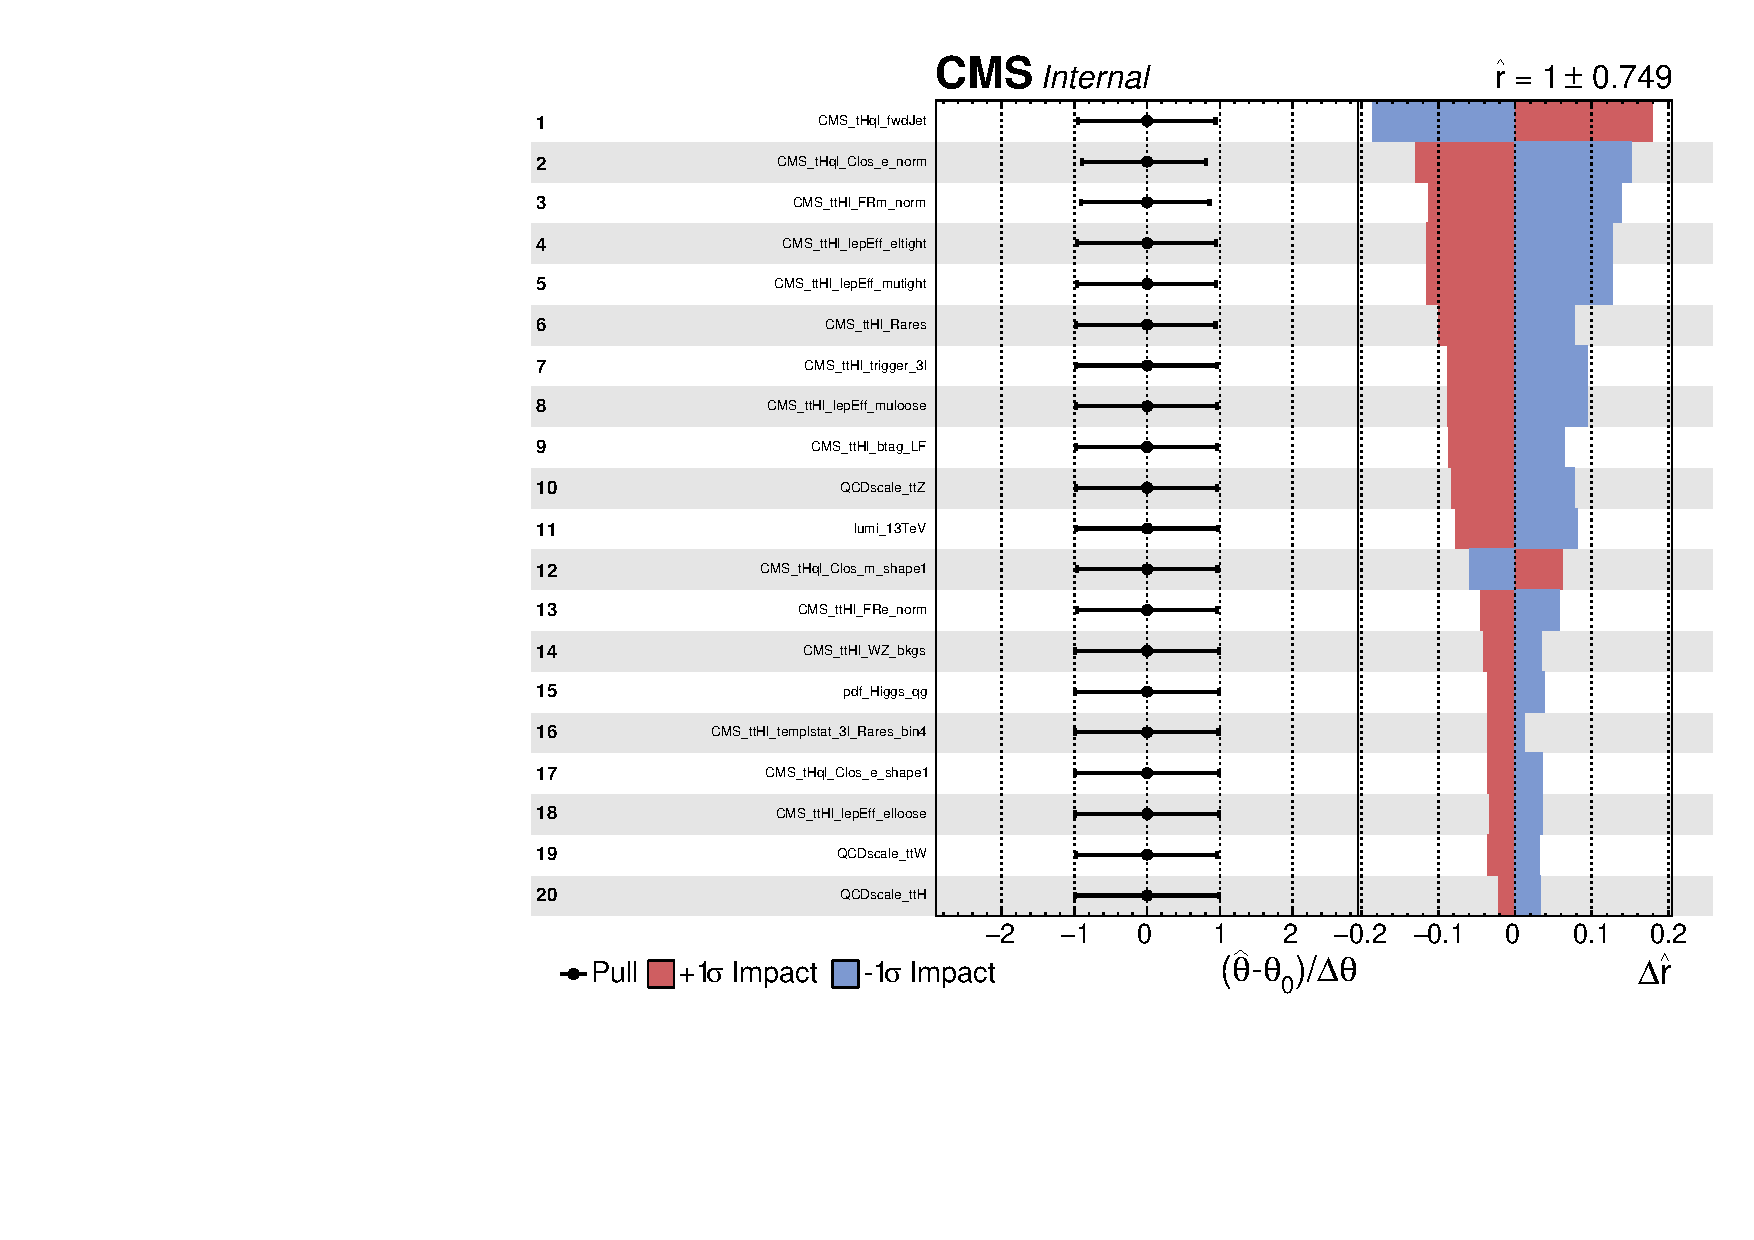
\includegraphics[width=1.0\textwidth]{limits/impacts/impacts_25.pdf}\\
\caption[Post-fit pulls and impacts with $\pt$ cut $25$ GeV for the forward jet]{Post-fit pulls and impacts of the 20 nuisance parameters with $\pt$ cut $25$ GeV for the forward jet.}
\label{fig:impact25}
\end{figure}

\begin{figure} [!h]
 \centering
 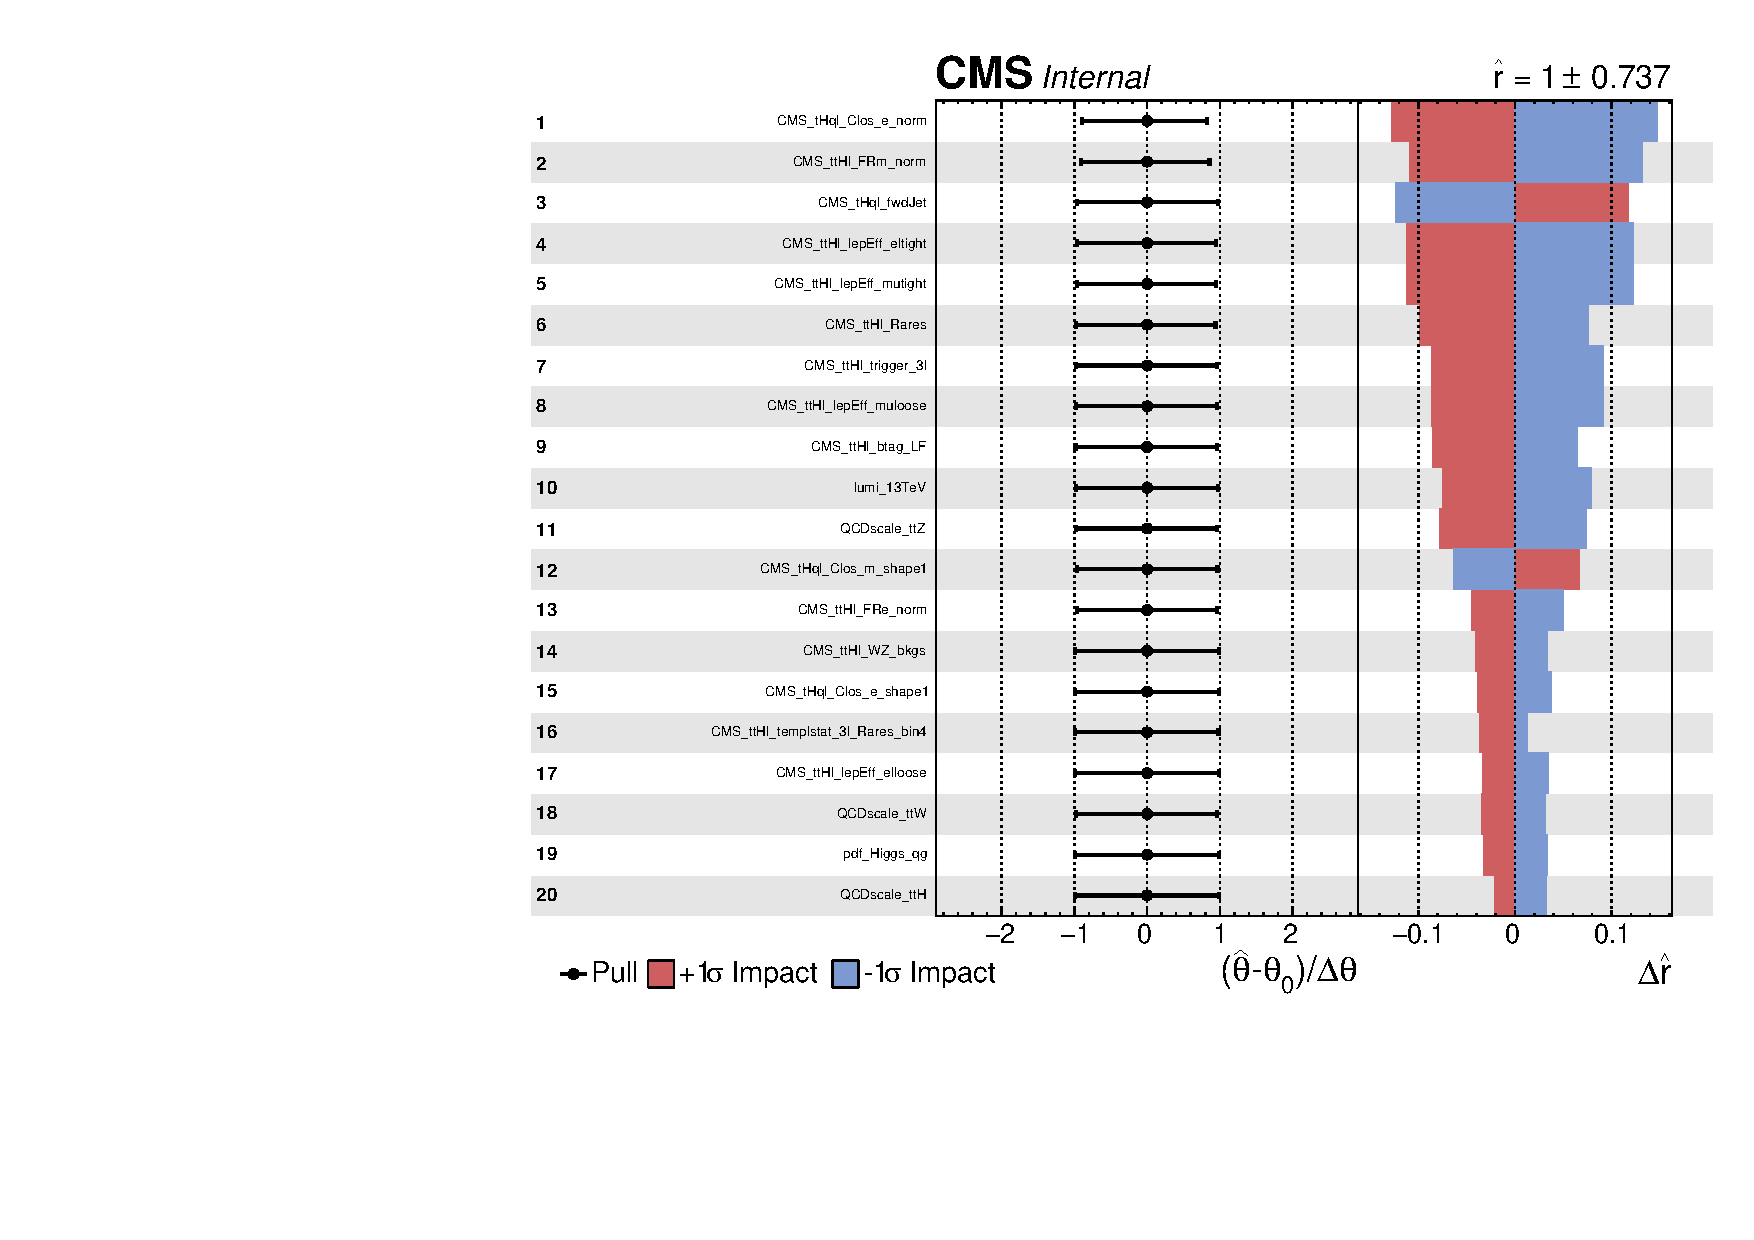
\includegraphics[width=1.0\textwidth]{limits/impacts/impacts_30.pdf}\\
\caption[Post-fit pulls and impacts with $\pt$ cut $30$ GeV for the forward jet]{Post-fit pulls and impacts of the 20 nuisance parameters with $\pt$ cut $30$ GeV for the forward jet.}
\label{fig:impact30}
\end{figure}

\begin{figure} [!h]
 \centering
 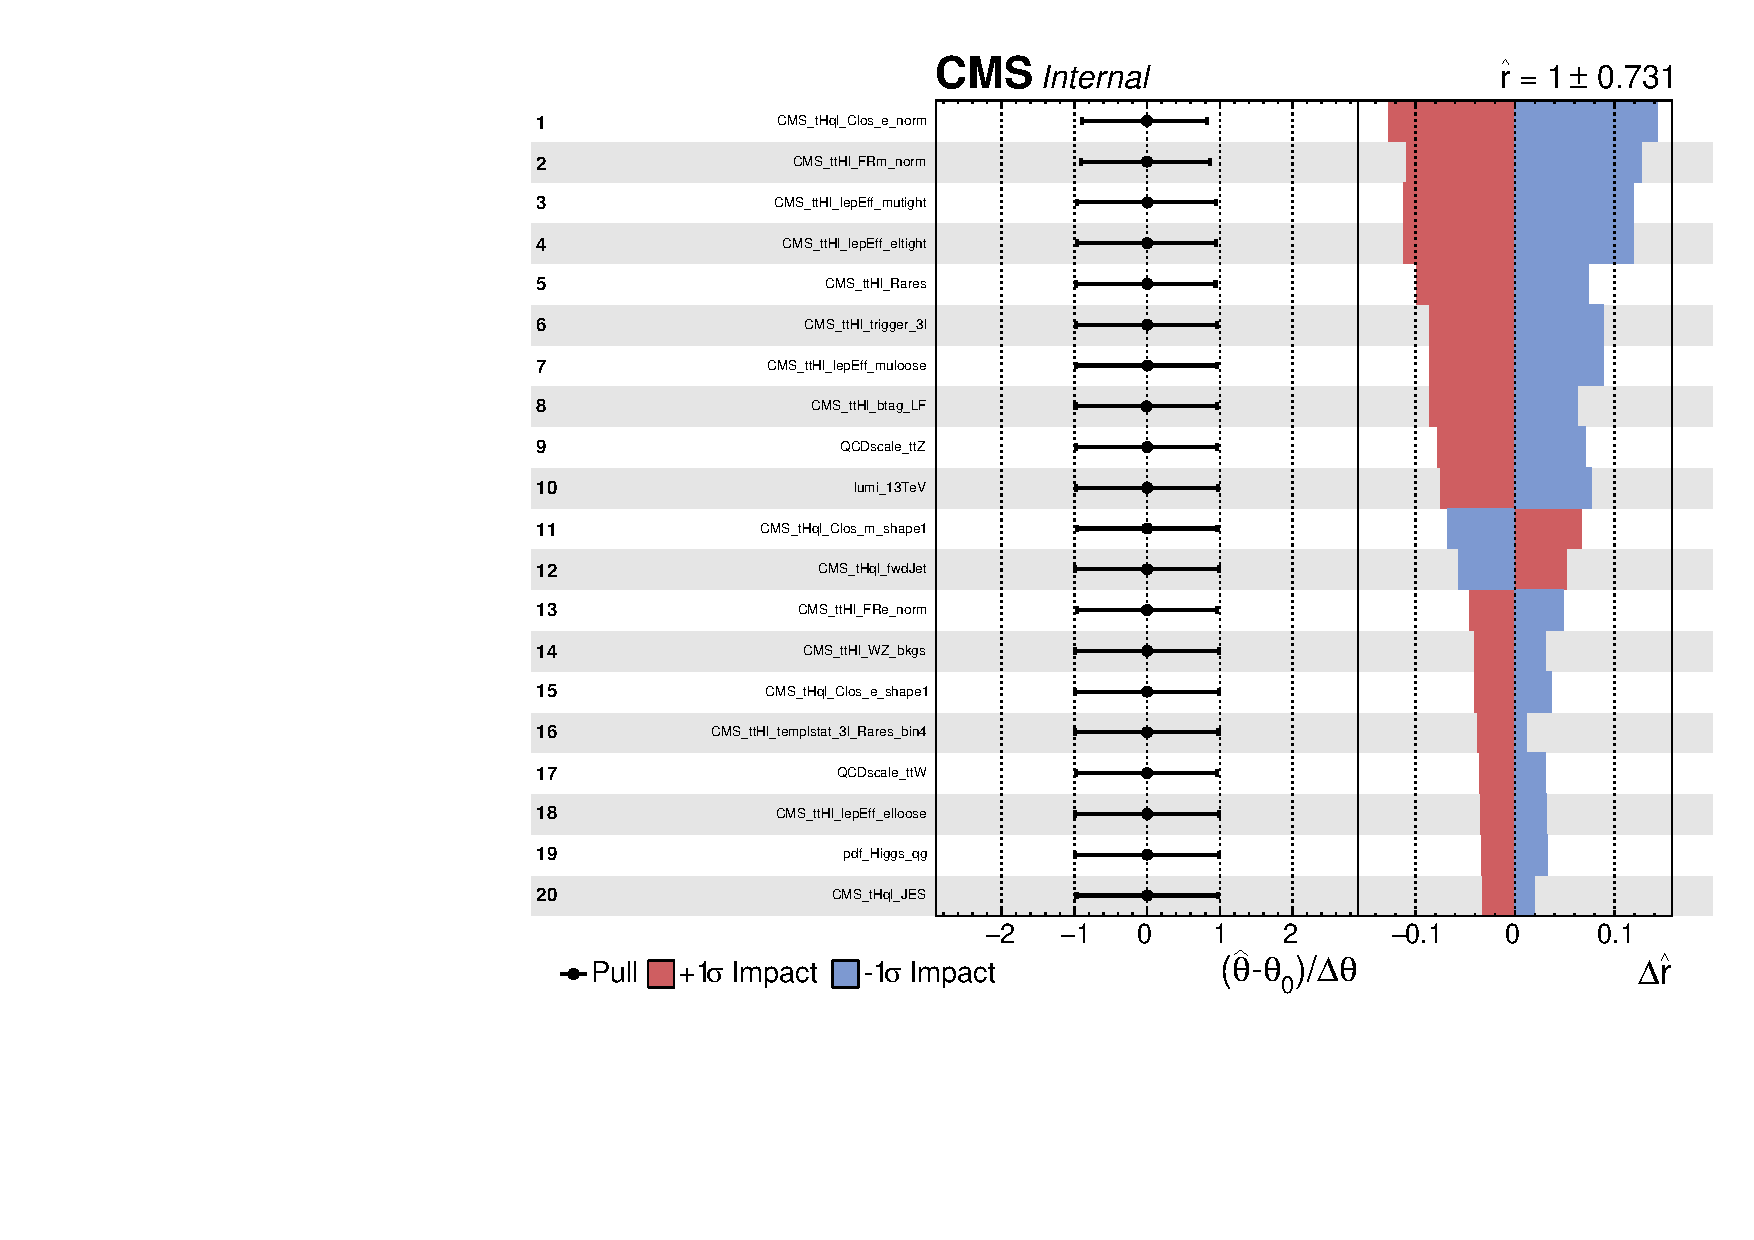
\includegraphics[width=1.0\textwidth]{limits/impacts/impacts_40.pdf}\\
\caption[Post-fit pulls and impacts with $\pt$ cut $25$ GeV for the forward jet]{Post-fit pulls and impacts of the 20 nuisance parameters with $\pt$ cut $40$ GeV for the forward jet.}
\label{fig:impact40}
\end{figure}
